%% Basierend auf einer TeXnicCenter-Vorlage von Mark Müller
%%%%%%%%%%%%%%%%%%%%%%%%%%%%%%%%%%%%%%%%%%%%%%%%%%%%%%%%%%%%%%%%%%%%%%%

% Wählen Sie die Optionen aus, indem Sie % vor der Option entfernen  
% Dokumentation des KOMA-Script-Packets: scrguide

%%%%%%%%%%%%%%%%%%%%%%%%%%%%%%%%%%%%%%%%%%%%%%%%%%%%%%%%%%%%%%%%%%%%%%%
%% Optionen zum Layout des Artikels                                  %%
%%%%%%%%%%%%%%%%%%%%%%%%%%%%%%%%%%%%%%%%%%%%%%%%%%%%%%%%%%%%%%%%%%%%%%%
\documentclass[%
%a5paper,							% alle weiteren Papierformat einstellbar
%landscape,						% Querformat
%10pt,								% Schriftgröße (12pt, 11pt (Standard))
%BCOR1cm,							% Bindekorrektur, bspw. 1 cm
%DIVcalc,							% führt die Satzspiegelberechnung neu aus
%											  s. scrguide 2.4
%twoside,							% Doppelseiten
%twocolumn,						% zweispaltiger Satz
%halfparskip*,				% Absatzformatierung s. scrguide 3.1
%headsepline,					% Trennline zum Seitenkopf	
%footsepline,					% Trennline zum Seitenfuß
%titlepage,						% Titelei auf eigener Seite
%normalheadings,			% Überschriften etwas kleiner (smallheadings)
%idxtotoc,						% Index im Inhaltsverzeichnis
%liststotoc,					% Abb.- und Tab.verzeichnis im Inhalt
%bibtotoc,						% Literaturverzeichnis im Inhalt
%abstracton,					% Überschrift über der Zusammenfassung an	
%leqno,   						% Nummerierung von Gleichungen links
%fleqn,								% Ausgabe von Gleichungen linksbündig
%draft								% überlangen Zeilen in Ausgabe gekennzeichnet
]
{scrartcl}

%\pagestyle{empty}		% keine Kopf und Fußzeile (k. Seitenzahl)
%\pagestyle{headings}	% lebender Kolumnentitel

%% Deutsche Anpassungen %%%%%%%%%%%%%%%%%%%%%%%%%%%%%%%%%%%%%
\usepackage[english]{babel}
\usepackage[T1]{fontenc}
\usepackage[utf8]{inputenc}

\usepackage{amsthm} % Theorem-Packet
\usepackage{amsmath}
\usepackage{amssymb}

\usepackage{stmaryrd} % Blitzsymbol
\usepackage{fancyhdr} % Für Kopfzeile
\usepackage{graphicx} % Einbinden von Grafiken
\usepackage{bbding} % Für das Häckchen
\usepackage{amscd} % Kommutative Diagramme
\usepackage{mathtools} % Für das Definitionssymbol

\usepackage{listings}
\usepackage{courier}

\pagestyle{fancy}
\lhead{Computational Science I}\chead{Exercise notes: Matrices}\rhead{HS 2013} % Kopfzeile

\newtheoremstyle{plain}%  name
  {.5\baselineskip}% Space above
  {.5\baselineskip}% Space below
  {}% Body font
  {}% Indent amount (empty = no indent, \parindent = para indent)
  {\bfseries}% Thm head font
  {:}% Punctuation after thm head
  { }% Space after thm head: " " = normal interword space; \newline = linebreak
  {}% Thm head spec (can be left empty, meaning `normal')
  
\makeatletter % Matrizen mit opitonalen Linien
\renewcommand*\env@matrix[1][*\c@MaxMatrixCols c]{%
  \hskip -\arraycolsep
  \let\@ifnextchar\new@ifnextchar
  \array{#1}}
\makeatother

\theoremstyle{plain}
\newtheorem*{bsp}{Beispiel} % Beispiele ohne Nummerierung
\newtheorem*{bws}{Beweis} % Beweise ohne Nummerierung 
\newenvironment{beweis}{\begin{bws}~\vspace{0.5\baselineskip}}{\hfill $\qedsymbol$\end{bws}}
\newenvironment{beispiel}{\begin{bsp}~\vspace{0.5\baselineskip}}{\end{bsp}}

\usepackage{lmodern} % Type1-Schriftart für nicht-englische Texte

\usepackage{enumerate}

\renewcommand\theenumi{\roman{enumi}}
\renewcommand\labelenumi{\theenumi)}

%% Packages für Grafiken & Abbildungen %%%%%%%%%%%%%%%%%%%%%%
%\usepackage{graphicx} %%Zum Laden von Grafiken
%\usepackage{subfig} %%Teilabbildungen in einer Abbildung
%\usepackage{tikz} %%Vektorgrafiken aus LaTeX heraus erstellen

%\setlength{\parindent}{0pt} % kein Einzug


%% Beachten Sie:
%% Die Einbindung einer Grafik erfolgt mit \includegraphics{Dateiname}
%% bzw. über den Dialog im Einfügen-Menü.
%% 
%% Im Modus "LaTeX => PDF" können Sie u.a. folgende Grafikformate verwenden:
%%   .jpg  .png  .pdf  .mps
%% 
%% In den Modi "LaTeX => DVI", "LaTeX => PS" und "LaTeX => PS => PDF"
%% können Sie u.a. folgende Grafikformate verwenden:
%%   .eps  .ps  .bmp  .pict  .pntg


%% Bibliographiestil %%%%%%%%%%%%%%%%%%%%%%%%%%%%%%%%%%%%%%%%%%%%%%%%%%
%\usepackage{natbib}

\begin{document}

\lstset{basicstyle=\ttfamily, breakatwhitespace=false, breaklines=true, frame=single, xleftmargin=\parindent, aboveskip=\baselineskip, belowskip=\baselineskip}

%\pagestyle{empty} %%Keine Kopf-/Fusszeilen auf den ersten Seiten.


%%%%%%%%%%%%%%%%%%%%%%%%%%%%%%%%%%%%%%%%%%%%%%%%%%%%%%%%%%%%%%%%%%%%%%%
%% Ihr Artikel                                                       %%
%%%%%%%%%%%%%%%%%%%%%%%%%%%%%%%%%%%%%%%%%%%%%%%%%%%%%%%%%%%%%%%%%%%%%%%

%% eigene Titelseitengestaltung %%%%%%%%%%%%%%%%%%%%%%%%%%%%%%%%%%%%%%%    
%\begin{titlepage}
%Einsetzen der TXC Vorlage "Deckblatt" möglich
%\end{titlepage}

%% Angaben zur Standardformatierung des Titels %%%%%%%%%%%%%%%%%%%%%%%%
\titlehead{\center{University of Zurich - HS 2013}}
%\subject{Typisierung}
\title{Computational Science I\\Exercise notes: Matrices\\\rule{1.0\textwidth}{1.0pt}}
\author{Tobias Grubenmann}
%\and{Der Name des Co-Autoren}
%\thanks{Fußnote}			% entspr. \footnote im Fließtext
%\date{}							% falls anderes, als das aktuelle gewünscht
%\publishers{Herausgeber}

%% Widmungsseite %%%%%%%%%%%%%%%%%%%%%%%%%%%%%%%%%%%%%%%%%%%%%%%%%%%%%%
%\dedication{Widmung}

\maketitle 						% Titelei wird erzeugt

%% Zusammenfassung nach Titel, vor Inhaltsverzeichnis %%%%%%%%%%%%%%%%%
%\begin{abstract}
% Für eine kurze Zusammenfassung des folgenden Artikels.
% Für die Überschrift s. \documentclass[abstracton].
%\end{abstract}

%% Erzeugung von Verzeichnissen %%%%%%%%%%%%%%%%%%%%%%%%%%%%%%%%%%%%%%%
%\tableofcontents			% Inhaltsverzeichnis
%\listoftables				% Tabellenverzeichnis
%\listoffigures				% Abbildungsverzeichnis


%% Der Text %%%%%%%%%%%%%%%%%%%%%%%%%%%%%%%%%%%%%%%%%%%%%%%%%%%%%%%%%%%

\section*{Exercise 1}

First, we need to get the equations for the resistor-cube problem:

\begin{eqnarray*}
\frac{V_{0}-V_{1}}{R_{01}}+\frac{V_{0}-V_{3}}{R_{03}}+\frac{V_{0}-V_{5}}{R_{05}}+I_{0}&=&0\\
\frac{V_{1}-V_{0}}{R_{01}}+\frac{V_{1}-V_{2}}{R_{12}}+\frac{V_{1}-V_{6}}{R_{16}}&=&0\\
\frac{V_{2}-V_{1}}{R_{12}}+\frac{V_{2}-V_{3}}{R_{23}}+\frac{V_{2}-V_{7}}{R_{27}}&=&0\\
\frac{V_{3}-V_{0}}{R_{03}}+\frac{V_{3}-V_{2}}{R_{23}}+\frac{V_{3}-V_{4}}{R_{34}}&=&0\\
\frac{V_{4}-V_{3}}{R_{34}}+\frac{V_{4}-V_{5}}{R_{45}}+\frac{V_{4}-V_{7}}{R_{47}}&=&0\\
\frac{V_{5}-V_{0}}{R_{05}}+\frac{V_{5}-V_{4}}{R_{45}}+\frac{V_{5}-V_{6}}{R_{56}}&=&0\\
\frac{V_{6}-V_{1}}{R_{16}}+\frac{V_{6}-V_{5}}{R_{56}}+\frac{V_{6}-V_{7}}{R_{67}}&=&0\\
\frac{V_{7}-V_{2}}{R_{27}}+\frac{V_{7}-V_{4}}{R_{47}}+\frac{V_{7}-V_{6}}{R_{67}}+I_{7}&=&0\\
\end{eqnarray*}

From this equations we get the following matrix equation:

\begin{equation*}
\begin{pmatrix}
(\frac{1}{R_{01}}+\frac{1}{R_{03}}+\frac{1}{R_{05}})&-\frac{1}{R_{01}}&0&-\frac{1}{R_{03}}&0&-\frac{1}{R_{05}}&0&0&1&0\\
&&&&&&&\\
&&&\vdots&&&&&&\\
&&&&&&&&&\\
&&&&&&&&&\\
&&&&&&&&&\\
&&&&&&&&&\\
&&&&&&&&&\\
1&0&0&0&0&0&0&0&0&0\\
0&0&0&0&0&0&0&1&0&0\\
\end{pmatrix}
\begin{pmatrix}V_{0}\\V_{1}\\V_{2}\\V_{3}\\V_{4}\\V_{5}\\V_{6}\\V_{7}\\I_{0}\\I_{7}\end{pmatrix}=
\begin{pmatrix}0\\0\\0\\0\\0\\0\\0\\0\\V_{0}\\V_{7}\end{pmatrix}
\end{equation*}

Now we can implement a Python script that evaluates the total resistance between the edges 0 and 7 given the values for the resistors as well as the voltages $V_{0}$ and $V_{7}$:

\lstinputlisting[language=Python]{../ResistorCubeProblem.py}

With the function \texttt{getTotalResistance} we can now calculate the total resistance of a cube where all resistors have $1\Omega$ and $V_{0}=0V$, $V_{1}=1V$. We get the a total resistance of $0.833333\Omega$.

\section*{Exercise 2}

The function \texttt{fft} recursively calculates the fast Fourier transform of a function $f$. The function \texttt{testFFT} calculates the FFT for the function $f=\frac{1}{1+x^{2}}$.

\lstinputlisting[language=Python]{../FFTRecursive.py}

The function gives the following output:

\begin{center}
\centering
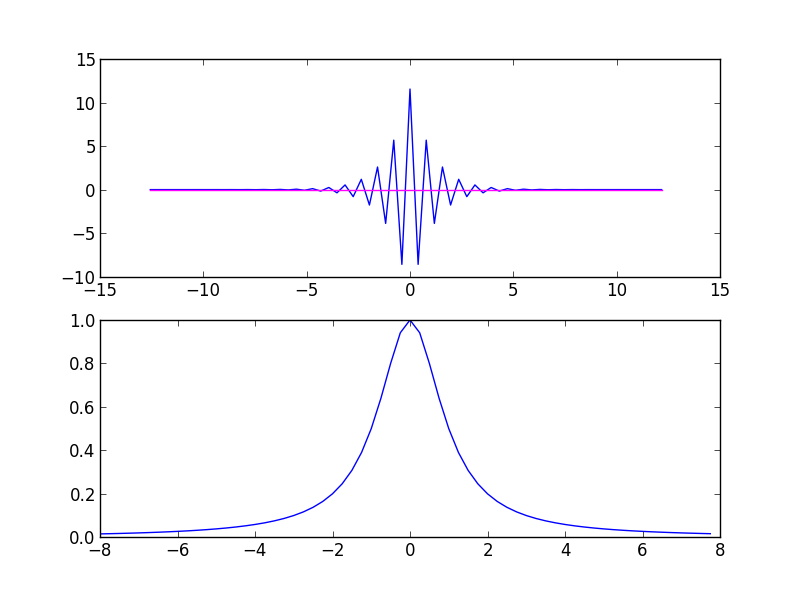
\includegraphics[width=0.6\linewidth]{../fft.png}
\captionof{figure}{FFT of $f=\frac{1}{1+x^{2}}$ with $N=64$.}
\end{center}

%% Bibliographie unter Verwendung von dinnat %%%%%%%%%%%%%%%%%%%%%%%%%%
%\setbibpreamble{Präambel}		% Text vor dem Verzeichnis
%\bibliographystyle{dinat}
%\bibliography{bibliographie}	% Sie benötigen einen *.bib-Datei

\end{document}


